\documentclass[11pt]{article} % 
\usepackage[pdftex]{graphicx}
\usepackage{fullpage}
\usepackage{graphicx}
\usepackage{graphics}
\usepackage{psfrag}
\usepackage{pgf}
\usepackage{color}
\usepackage{tikz}
\usetikzlibrary{arrows,automata}
\usepackage[latin1]{inputenc}
\usepackage{amsthm}
\usepackage{amsmath,amssymb}
\usepackage{enumerate}
\setlength{\textwidth}{6.5in}
\setlength{\textheight}{9in}
\newcommand{\N}{\mathbb{N}}
\newcommand{\Z}{\mathbb{Z}}
\newcommand{\R}{\mathbb{R}}
\newcommand{\Q}{\mathbb{Q}}
\newcommand{\C}{\mathbb{C}}
\newcommand{\PP}{\mathbb{P}}
\newcommand{\tab}{\;\;\;\;\;}
\newcommand{\inv}{^{-1}}
\newcommand{\tr}{\textrm}
\newcommand{\lc}{\sqcup}
\newcommand{\var}{\tr{Var}}
\newcommand{\cov}{\tr{Cov}}
\newcommand{\like}{\mathcal{L}}

\begin{document}

\hfill Robert Johns

\hfill February 27, 2014

\begin{center} {\Large CSCI 678: Statistical Analysis of Simulation Models}\\{\large Homework 6}\end{center}

\begin{enumerate}

%1
\item The maximum period is 10, the minimum is two. There are four sequences, two with two starting pairs, and two with five.  Those sequences are:

1, 4, (1, 4, ...)

2, 3, (2, 3, ...)

3, 1, 0, 4, 2, 2, 4, 0, 1, 3, (3, 1, ...)

1, 1, 2, 0, 3, 4, 4, 3, 0, 2, (1, 1, ...)

%%%%%
%2
\item Page 398 in the book tells us that, if parameters are chosen properly, a period of $m^2-1$ becomes possible.  

%%%%%
%3
\item We have from page 4.7 in the notes that an LCG $Z_i = (aZ_{i-1}+c)\mod m$ has a full period iff $c$ is odd, $m = 2^b$, and $a = 1\mod 4$.  We use that fact on the first three examples, and use the rules on page 4.6 for the last one.

\begin{enumerate}

%3a
\item $a = 13, c = 13, m = 16$.  All four criterion are satisfied, so we're good to go.

%3b
\item $a = 12, c = 13, m = 16$. $a \not= 1\mod 4$, so the generator does not have a full period.

%3c
\item $a = 13, c = 12, m = 16$.  $c$ is not odd, so the generator does not have a full period.

%3d
\item $a = 1, c = 12, m = 13$.  This satisfies the three rules on page 4.6, so it has a full period.

\end{enumerate}

%%%%%
%4
\item Marsaglia's Theorem only gives results for when $c = 0$, but he says ``similar results can be established for [when $c > 0$]" so I'll just use his.

\begin{enumerate}

%4a
\item Generator: $a = 5, c = 3, m = 16$ has a full period. If $n = 2, (n!m)^{1/n} = \sqrt{32} \approx 5.66$

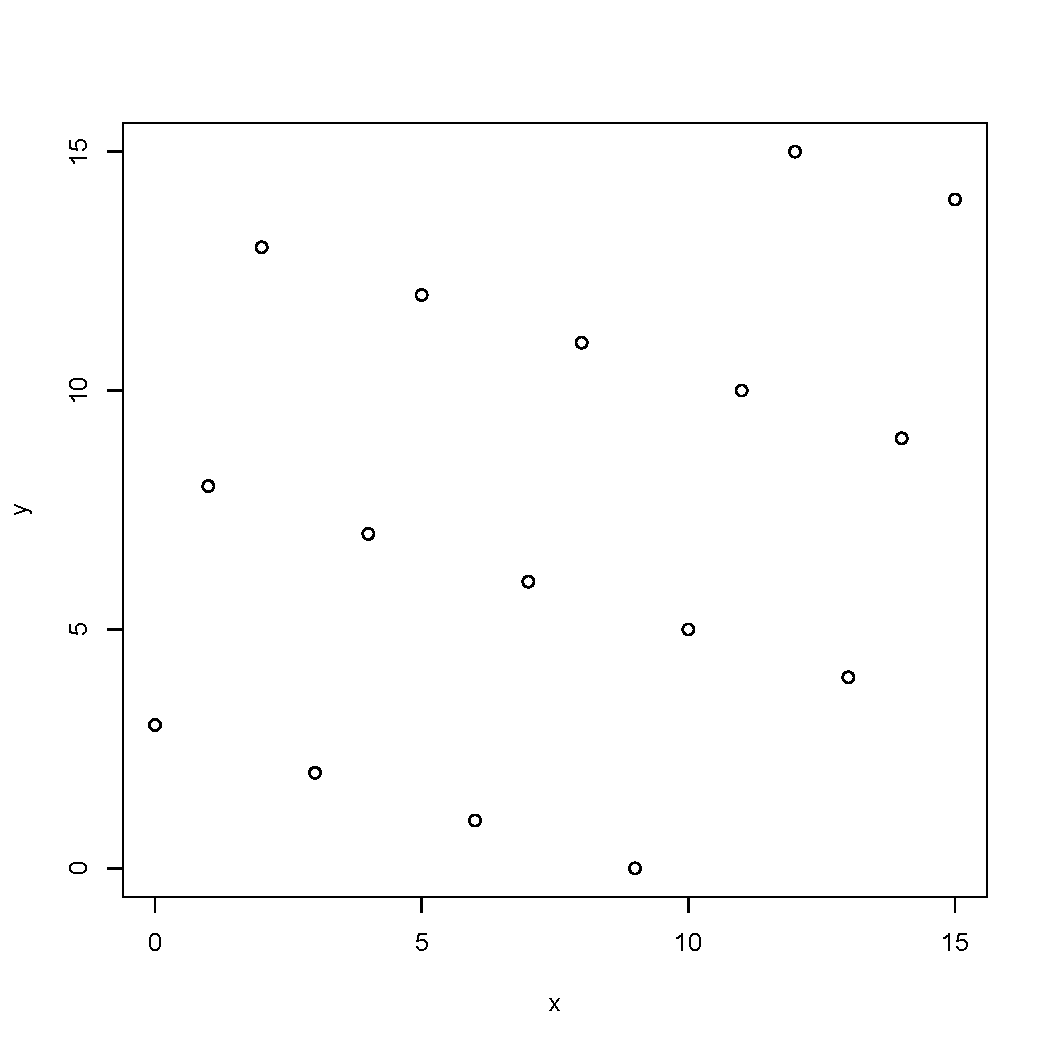
\includegraphics[scale = .4]{plot1.pdf}

We see that all points seem to fall into four lines more than 1 fewer than predicted by Marsaglia.

%4b
\item Generator: $a = 1, b = 12, m = 13$ has a full period.  If $n = 2, (n!m)^{1/n} = \sqrt{26} \approx 5.10$

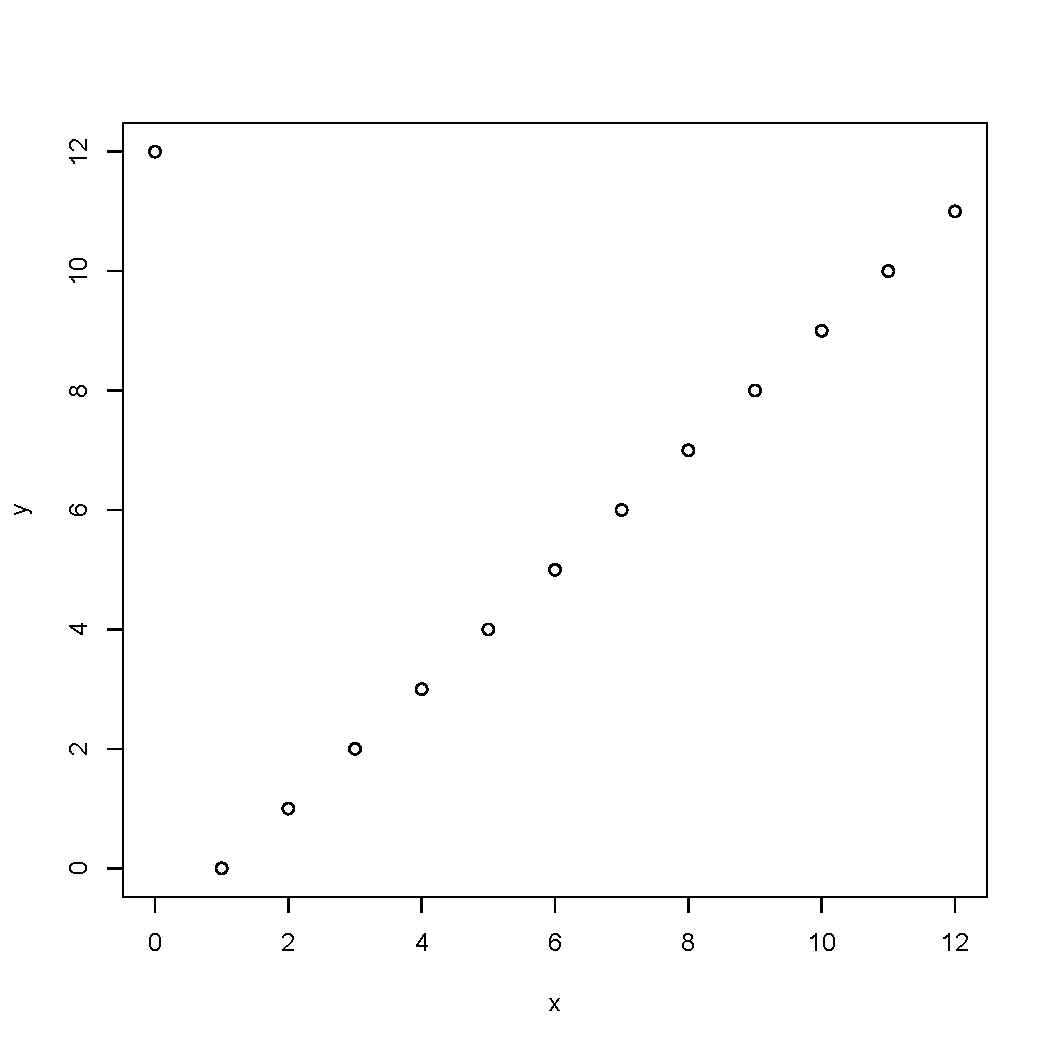
\includegraphics[scale = .4]{plot2.pdf}

All the points fall into two lines (all but one into one of them), more than 3 fewer than Marsaglia predicted.

\end{enumerate}

%%%%%
%5
\item \begin{enumerate}

%5a
\item If we let $c_1 = 1, c_2 = 6$, we see that $c_1 + 2c_2 = 1 + 12 = 13 = 0\mod13$.

%5b
\item If we examine

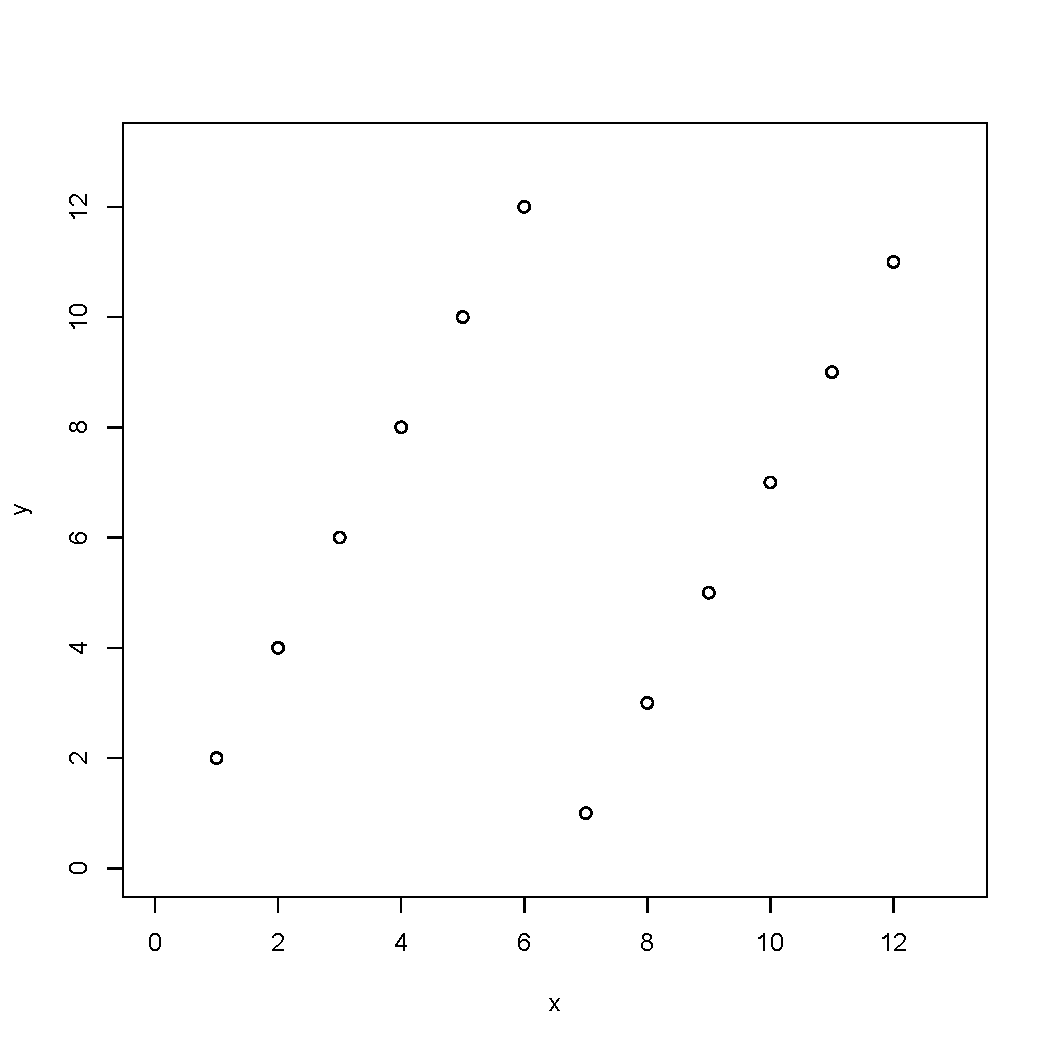
\includegraphics[scale = .4]{plot3.pdf}

we see that all $(U_i, U_{i+1})$ pairs lie in the appropriate lines.

\end{enumerate}

%%%%%
%6
\item The system will fail at the first failure of a component, so we're looking to generate the first order statistic of a Weibull(3,4).  We can do this randomly, without sorting, using the equations on 5.8 in the notes:
$$x_{(1)} = F\inv(u_{(1)}) = F\inv(1 - (1 - u)^{1/789}) = -4\sqrt[3]{\ln[(1 - u)^{1/789}]}$$

The program \texttt{asm6d.r} was used to calculate the mean and compute the output. The system has a mean failure time (after one run of 200 simulations) of $0.09340126$.  The file \texttt{output.txt}, attached at end, contains the 200 variates and the mean. The histogram is below:

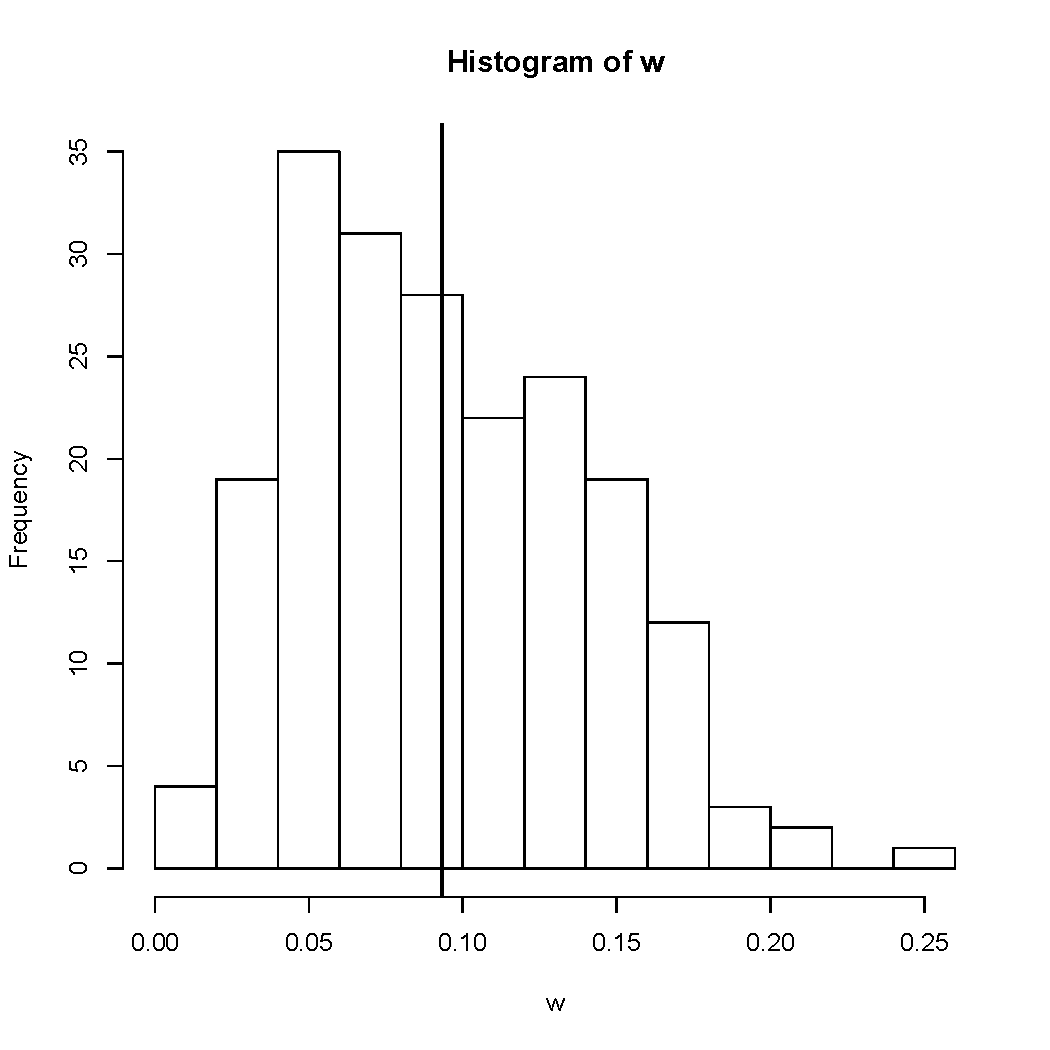
\includegraphics[scale = .4]{plot4.pdf}

The theoretical mean computation is attached at the end on a separate sheet.

%%%%%
%7
\item  The scatterplot follows:

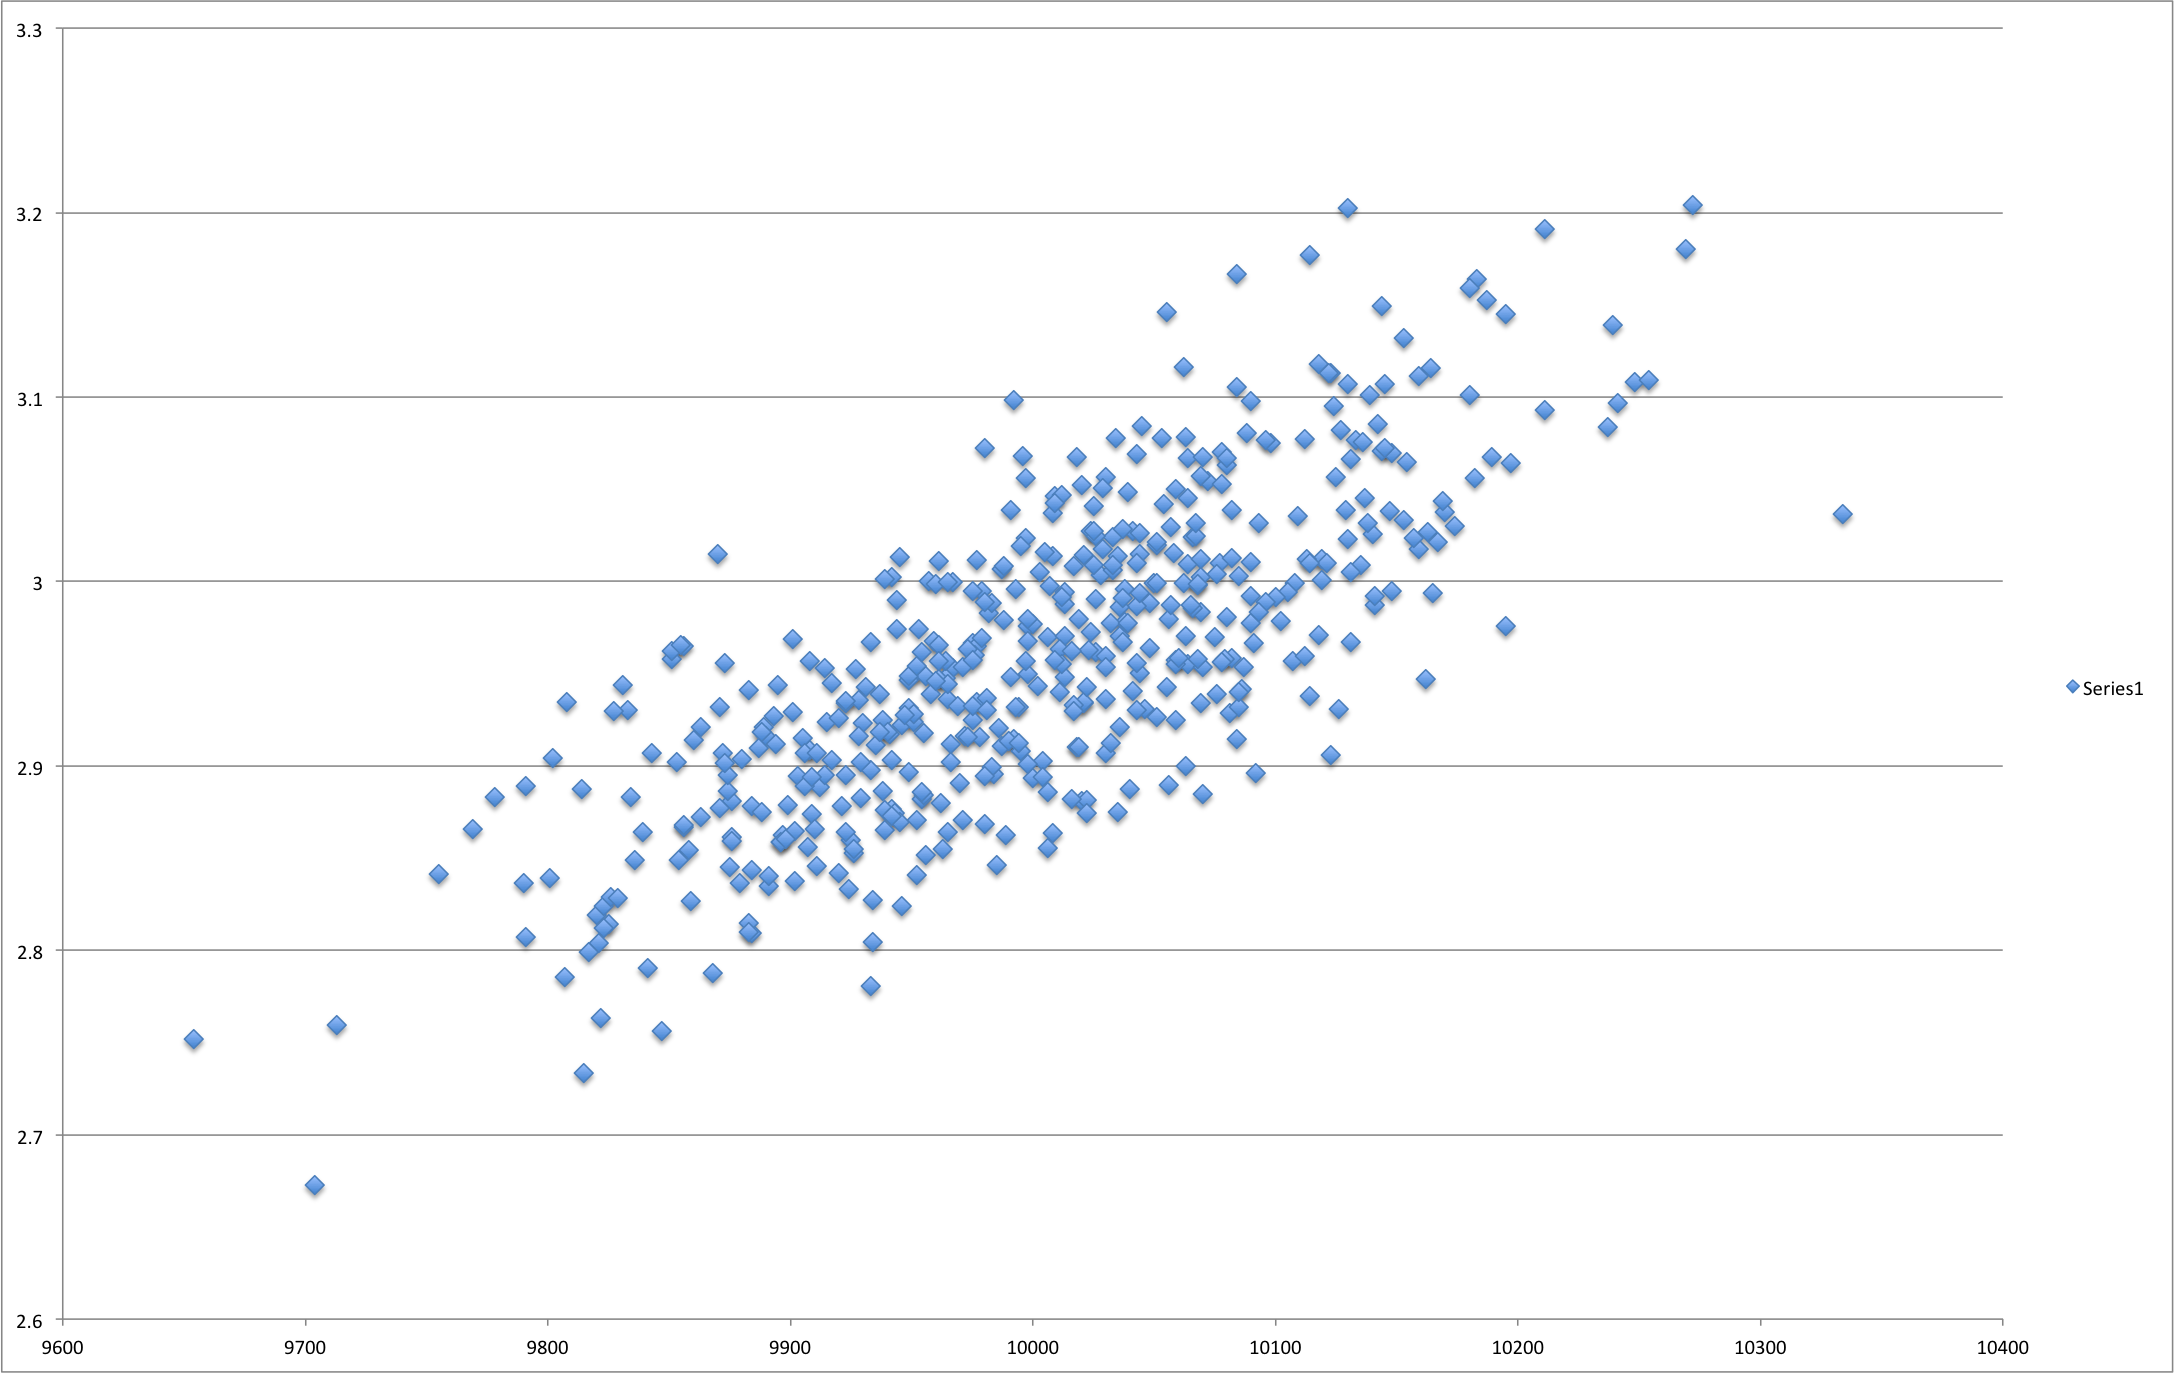
\includegraphics[scale = .45]{chart.png}

There seems to be a relatively strong correlation between number of jobs processed and wait time.  On the surface, this seems counterintuitive: if the number of jobs is lower, then the jobs got through the line faster and there was less wait.  Upon reflection, though, it becomes clear that due to the way the program is structured, if a job takes a long time, thus making the others wait longer, then more jobs will have time to arrive and so the simulation will keep going, ending with more jobs processed.

\end{enumerate}

\end{document}